\documentclass[crop,tikz]{standalone}
\usepackage{tikz-3dplot}
\usetikzlibrary{decorations.markings, backgrounds, calc}
\tikzset{>=latex}
\tikzset{->-/.style={decoration={
    markings,
    mark=at position .5 with {\arrow{>}} },postaction={decorate}}
}

\tikzset{-./.style={decoration={
    markings,
    mark=at position 1 with {\pgfuseplotmark{*}} },postaction={decorate}}
}

\tikzset{->-./.style={decoration={
    markings,
    mark=at position 0.6 with {\arrow{>}},
    mark=at position 1 with {\pgfuseplotmark{*}}
    },postaction={decorate}}
}

\tikzset{-<-./.style={decoration={
    markings,
    mark=at position 0.6 with {\arrow{<}},
    mark=at position 1 with {\pgfuseplotmark{*}}
    },postaction={decorate}}
}
\begin{document}
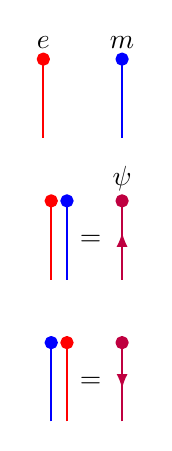
\begin{tikzpicture}[line join = round]
\draw[-.,red, thick] (0,0) -- +(0,1) node[anchor=south, black] (e) {$e$};
\draw[-.,blue, thick](1,0) -- +(0,1) node[anchor=south, black] (m) {$m$};


\draw[-.,red, thick] (0.1,-1.8) -- +(0,1);
\draw[-.,blue, thick](0.3,-1.8) -- +(0,1);
\node[anchor=center] at (0.6, -1.3) {$=$};
\draw[->-.,purple, thick](1.0,-1.8) -- +(0,1) node[anchor=south, black] (psi) {$\psi$};

\draw[-.,blue, thick] (0.1,-3.6) -- +(0,1);
\draw[-.,red, thick](0.3,-3.6) -- +(0,1);
\node[anchor=center] at (0.6, -3.1) {$=$};
\draw[-<-.,purple, thick](1.0,-3.6) -- +(0,1);

\end{tikzpicture}

\end{document} 
